%%% Template for documenting projects which involve circuit illustrations and code.
% Author: Claudiu Groza

% Template based on the template created by:
% Author:   Luis José Salazar-Serrano
%           totesalaz@gmail.com / luis-jose.salazar@icfo.es
%           http://opensourcelab.salazarserrano.com


\documentclass[a4paper,11pt]{article}

\usepackage[T1]{fontenc}
\usepackage[utf8]{inputenc}
\usepackage{graphicx}
\usepackage{xcolor}

\renewcommand\familydefault{\sfdefault}
\usepackage{tgheros}
\usepackage[defaultmono]{droidmono}

\usepackage{amsmath,amssymb,amsthm,textcomp}
\usepackage{enumerate}
\usepackage{multicol}
\usepackage{tikz}
\usepackage{courier}

\usepackage{pythonhighlight}

\usepackage{hyperref}

\usepackage{geometry}
\geometry{total={210mm,297mm},
left=25mm,right=25mm,%
bindingoffset=0mm, top=20mm,bottom=20mm}


\linespread{1.3}

\newcommand{\divider}{\rule{\linewidth}{0.5pt}}

% my own titles
\makeatletter
\renewcommand{\maketitle}{
\begin{center}
\vspace{2ex}
{\huge \textsc{\@title}}
\vspace{1ex}
\\
\divider\\
\@author \hfill \@date
\vspace{4ex}
\end{center}
}
\makeatother
%%%

% custom footers and headers
\usepackage{fancyhdr}
\pagestyle{fancy}
\lhead{}
\chead{}
\rhead{}
\lfoot{Temperature and Humidity Monitoring System}
\cfoot{}
\rfoot{Page \thepage}
\renewcommand{\headrulewidth}{0pt}
\renewcommand{\footrulewidth}{0pt}
%

% code listing settings
\usepackage{listings}

\lstset{%
  language = Octave,
  backgroundcolor=\color{white},   
  basicstyle=\footnotesize\ttfamily,       
  breakatwhitespace=false,         
  breaklines=true,                 
  captionpos=b,                   
  commentstyle=\color{gray},    
  deletekeywords={...},           
  escapeinside={\%*}{*)},          
  extendedchars=true,              
  frame=single,                    
  keepspaces=true,                 
  keywordstyle=\color{orange},       
  morekeywords={*,...},            
  numbers=left,                    
  numbersep=5pt,                   
  numberstyle=\footnotesize\color{gray}, 
  rulecolor=\color{black},         
  rulesepcolor=\color{blue},
  showspaces=false,                
  showstringspaces=false,          
  showtabs=false,                  
  stepnumber=2,                    
  stringstyle=\color{orange},    
  tabsize=2,                       
  title=\lstname,
  emphstyle=\bfseries\color{blue}%  style for emph={} 
} 

%%%----------%%%----------%%%----------%%%----------%%%

\begin{document}

\title{Temperature and Humidity Monitoring System}

\author{Joe Doe, John Doe, Politehnica University of Timisoara}

\date{June, 2018}

\maketitle


\textit{The purpose of this document is to provide a comprehensive documentation template.\\
Some sections from the overall information might be dummy but it helps to emulate specific concerns.
Paragraphs formatted using the italic style provide in-place advice. They should not be contained in your project documentation.
Provided LATEX source file should be used as base format to write your documentation.
}

\section{Repository}
\textit{Related files to your work must be placed within a version control system. I strongly suggest to use Github but any git system should just be fine.}\\\\
Schematics, diagrams and codebase are contained under the following git repository:\\
\textbf{\url{https://github.com/claudiugroza/msa}}

\section{User requirements}
\textit{Imagine talking to a person without any technical background. User requirements should express the intentions of a common user and not how you plan to engineer the system.}

\begin{enumerate}  
\item The system must provide information relevant to temperature and humidity in a certain area.
\item The system should be open for extension, eg. adding a barometer.
\item The system should run in an environment that provides a 24/24 access.
\item Temperature and humidity information should be accessed via a Web interface or a mobile application.
\item The system must provide the current temperature and humidity. The maximum
latency should be 10 seconds.
\item The system might provide access to history data for the last 2 weeks.
\item The system may provide a module for data interpretation.
\end{enumerate}

\section{System overview}
\textit{Illustrate how you engineered the system from a generic point of view. You should point out all the important subsystems, modules or entities.}\\

The overview of the system is depicted in Figure \ref{fig:system}.

\begin{figure}[h]
\centering
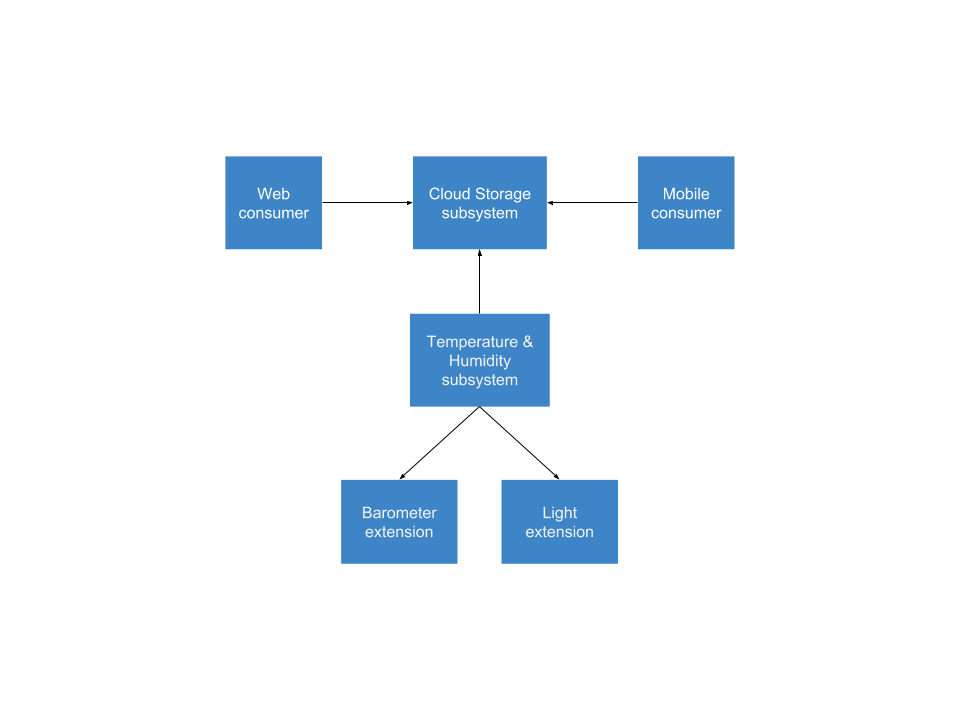
\includegraphics[scale=0.5]{system-overview.png}
\caption{System overview diagram}
\label{fig:system}
\end{figure}

Base (Temperature \& Humidity) Subsystem encompasses the measurement functionality. It has the sole purpose to acquire information from it’s sensors and extensions.\\

Barometer extension provides an interface for pressure querying. It must conform to an interface defined by the Base Subsystem.\\

Light extension provides an interface for light related data. It must implement the interface defined by the Base Subsystem.\\

Cloud Storage Subsystem stores the data pushed by the Base Subsystem. Additionally, it offers a possibility to interpret stored information.\\

Web consumer provides a UI interpretation for the data stored in the Cloud Storage Subsystem. This view is accessed within a Web browser.\\

Mobile consumer also provides a UI interpretation for the stored data. The view will be accessed via a specialised application which runs on a mobile device.

\section{Circuit design}
\textit{Provide a detailed perspective of the hardware components you’ve used in your project. You can use Fritzing tool to draw the schematics.}\\

The hardware view of the system is depicted in Figure \ref{fig:circuit-design}.

\begin{figure}[h]
\centering
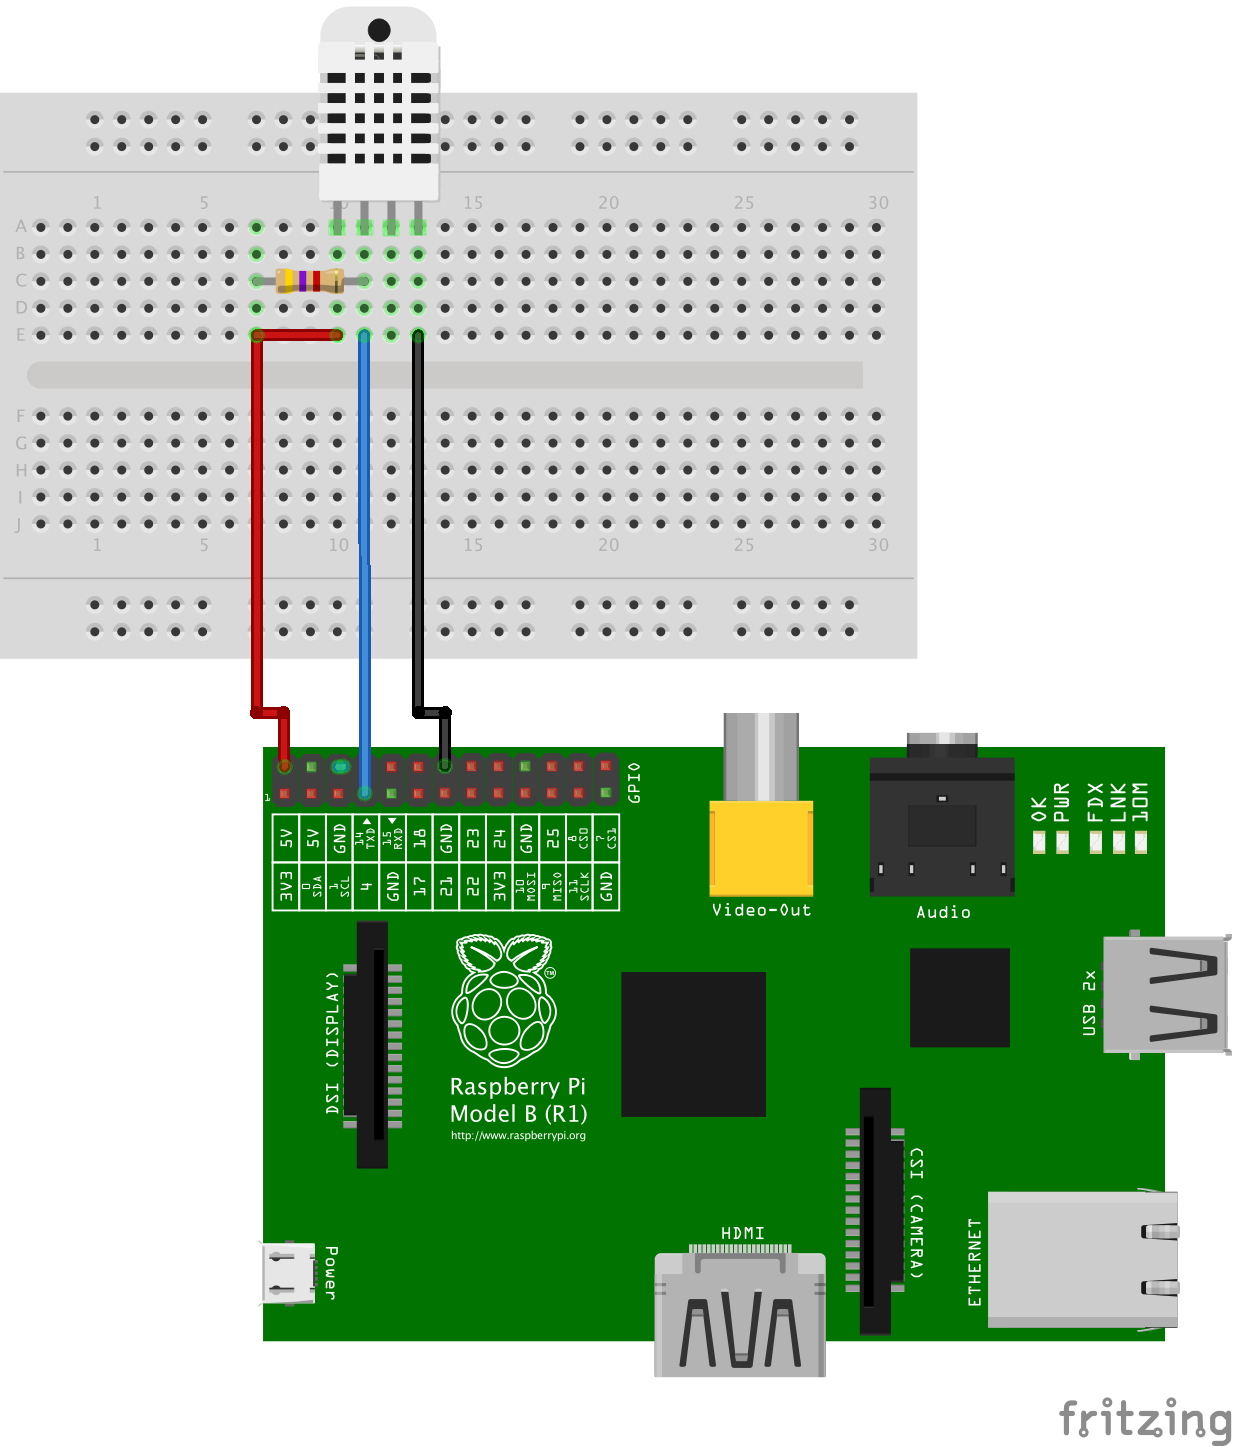
\includegraphics[scale=0.7]{circuit-design.png}
\caption{Circuit schematic}
\label{fig:circuit-design}
\end{figure}

Raspberry Pi 2 provides support for quick prototyping. That makes it a perfect choice for quick prototyping but not adequate for real-time applications. We will use the one-wire interface it has, but also the implicit possibility of communicating with other devices over the Internet. \\

AM2302 (DHT-22) is an one-wire enabled sensor. It is a basic, digital-output relative temperature and humidity sensor.\\

The wiring of the components can be observed in Figure \ref{fig:circuit-design}. An important aspect we need to mention is that the communication between the board and sensor is done via the one-wire interface.


\section{Software design}
\textit{Provide a walktrough of the most important components/modules/entities or concepts you've implemented in the software section.}\\

The software components and data flow directions are depicted in Figure \ref{fig:soft-design}. Each of these will be presented in the following subsections.\\

\begin{figure}[h]
\centering
\includegraphics[scale=0.7]{soft-design.png}
\caption{Software entities involved}
\label{fig:soft-design}
\end{figure}
 
\subsection{Python modules}
\textit{You should not concentrate on providing line level descriptions, but rather class/script/module level explanations. Short code comments are strongly advised. Third party libraries should also have a brief description and a reference link.}\\

write\_firebase\_sensor.py: it retrieves the temperature and humidity tuple from DHT-22 sensor over the one-wire interface and then pushes it to Firebase every 1 second. \\

Adafruit\_DHT22 library: it provides a quick implementation of one-wire interface communication with the sensor.

\subsection{Firebase}
\textit{Describe the purpose of the service and present the specifics you are using.}\\

Firebase is a PaaS (Platform as a Service) which means it offers developers to a quick list of functionalities supported by a traditional backend.
Realtime Database simplifies storing and synchronising data between different devices in realtime using a noSQL database.

The following code section shows the initialization of the Firebase project.

\newpage
\begin{python}
# the generated root for your project
FIREBASE_ROOT = 'https://ms-iot.firebaseio.com'
# init Firebase Database instance
firebase = firebase.FirebaseApplication(FIREBASE_ROOT, None)
\end{python}

\subsection{Android application}
\textit{Explain the responsibility of some key entities contained in your Android project.}

\subsection{Android application}
\textit{Give a brief description of the main parts contained by the JavaScript module.}

\section{Results and further work}
\textit{Describe what you accomplished so far, then what you plan to improve or extend.}\\

The current version of the project supports the following functionalities:
\begin{itemize}  
\item reliable reading of the temperature and humidity
\item storing data to Firebase Database
\item client implementations for retrieving data stored in Firebase Database (Android and WEB)\\
\end{itemize}

The following list of extensions and improvements was identified to be supported in the future:
\begin{itemize}  
\item remote access for configuring temperature and humidity interval reading
\item extend Android app functionality to display retrieved information in real-time diagrams
\item extend JavaScript application to support .csv exports
\item improve the hierarchy design of Firebase Database
\end{itemize}

\newpage
\section{References}
\begin{enumerate}  
\item Draw IO [last seen: May 2018], \url{https://www.draw.io/}
\item Fritzing [last seen: May 2018], \url{http://fritzing.org/}
\item Firebase Database [last seen: May 2018], \url{https://firebase.google.com/docs/database/}
\item DHT22Datasheet [last seen: May 2018], \url{https://cdn-shop.adafruit.com/datasheets/Digital+humidity+and+temperature+sensor+AM2302.pdf}
\item AdafruitDHT library [last seen: May 2018], \url{https://github.com/adafruit/Adafruit\_Python\_DHT}
\end{enumerate}



\end{document}
